\chapter{Τετραγωνικός Προγραμματισμός}\label{ch:qp}
Μία ειδική κατηγορία μη-γραμμικού προγραμματισμού παρουσιάζεται όταν η
αντικειμενική συνάρτηση $f$ είναι τετραγωνική και οι περιορισμοί είναι
γραμμικοί. Τότε το πρόβλημα ονομάζεται \textbf{Τετραγωνικός Προγραμματισμός} και
είναι της μορφής
\begin{equation}\label{eq:qp_min}
    \begin{aligned}
        & \underset{x}{\text{\tl{min}}}
        & & q(x) = \frac{1}{2}x^TGx + x^Tc \\
        & \text{\tl{subject to}}
        & & a^T_ix = b_i, \quad i \in \mathcal{E}, \\
        &&& a_i^Tx \ge b_i, \quad i \in \mathcal{I},
    \end{aligned}
\end{equation}
όπου $G$ είναι $n \times n$ συμμετρικό μητρώο, $\mathcal{E}$ και $\mathcal{I}$
είναι πεπερασμένα σύνολα των δεικτών, και $c, x,$ και $\{a_i\}, i \in
\mathcal{E}\cup \mathcal{I}$, είναι διανύσματα στο $\mathbb{R}^n$. Τετραγωνικά
προγράμματα μπορούν να λυθούν αριθμητικά (αν έχουν λύση) και η δυσκολία να
βρεθεί λύση εξαρτάται από τα χαρακτηριστικά της αντικειμενικής συνάρτησης και
τον αριθμό των περιορισμών. Έχουν αναπτυχθεί πολλές μέθοδοι επίλυσης προβλημάτων
τετραγωνικού προγραμματισμού που περιέχουν περιορισμούς ισότητας και ανισότητας.
Οι μέθοδοι ενεργών περιορισμών (\tl{active set}) χρησιμοποιούνται ευρέως από το
$1970$ και είναι αποτελεσματικοί για μικρό και μεσαίου μεγέθους προβλήματα.
Επιτρέπουν αποτελεσματική ανίχνευση της μη φραγμένης λύσης και τη μη εφικτότητας
και γενικά επιστρέφουν μία ακριβή εκτίμηση της βέλτιστης λύσης. Οι μέθοδοι
εσωτερικού σημείου (\tl{interior point}) είναι πιο πρόσφατοι και έγιναν
ιδιαιτέρως διάσημοι από το $1990$ και μετά. Είναι κατάλληλοι για μεγάλου
μεγέθους προβλήματα αλλά μπορεί να μην είναι οι πιο αποδοτικοί όταν θέλουμε να
λύσουμε παρόμοια τετραγωνικά προγράμματα, ο ενδιαφερόμενος αναγνώστης παραπέμπεται στο
\cite{boyd2004convex}. Μία άλλη μέθοδος είναι η προβολή
κλίσης (\tl{gradient projection}) και πρόκειται για ειδική περίπτωση της
μεθόδου των ενεργών περιορισμών, που είναι περισσότερο αποδοτική όταν οι μόνοι
περιορισμοί είναι τα όρια στις μεταβλητές. Στην παρούσα εργασία θα παρουσιάσουμε την
μέθοδο των ενεργών περιορισμών σύμφωνα με τη βοήθεια του
\cite{nocedal2006numerical}.

\section{Τετραγωνικό πρόγραμμα με περιορισμούς ισότητας}\label{sec:qp_eq}
Ξεκινάμε αναφέροντας την ειδική περίπτωση του γενικού προβλήματος
\eqref{eq:qp_min}, καθώς πολλοί αλγόριθμοι λύνουν σε κάθε
επανάληψη ένα υποπρόγραμμα με περιορισμούς ισότητας. Το τετραγωνικό πρόγραμμα
μπορεί να γραφτεί σε μητρωική μορφή
\begin{equation}\label{eq:qp_min_eq}
    \begin{aligned}
        & \underset{x}{\text{\tl{min}}}
        & & q(x) := \frac{1}{2}x^TGx + x^Tc \\
        & \text{\tl{subject to}}
        & & Ax = b,
    \end{aligned}
\end{equation}
όπου $A$ είναι η $m\times n$ Ιακωβιανή των περιορισμών με γραμμές τα $a_i^T, i
\in \mathcal{E}$ και $b$ είναι διάνυσμα στο $\mathbb{R}^m$ με συνιστώσες τα
$b_i, i \in \mathcal{E}$.

Οι πρώτης τάξης αναγκαίες συνθήκες για να είναι το $x^*$ λύση του
\eqref{eq:qp_min_eq} τότε υπάρχει διάνυσμα $\lambda^*$ τέτοιο ώστε να
ικανοποιείται το σύστημα
\begin{equation*}
    \begin{pmatrix}
        G & -A^T \\
        A & 0
    \end{pmatrix}
    \begin{pmatrix}
        x^* \\
        \lambda^*
    \end{pmatrix}=
    \begin{pmatrix}
        -c \\
        b
    \end{pmatrix}.
\end{equation*}
Το διάνυσμα $\lambda^*$ ονομάζονται πολλαπλασιαστές \tl{Lagrange}. Το παραπάνω
σύστημα μπορεί να γραφτεί σε μορφή βολική για τον υπολογισμό εκφράζοντας το
$x^*$ ως $x^* = x + p$, όπου $x$ είναι μία εκτίμηση της λύσης και $p$ είναι το
επιθυμητό βήμα. Με αυτόν το συμβολισμό προκύπτει
\begin{equation}\label{eq:qp_kkt}
    \begin{pmatrix}
        G & -A^T \\
        A & 0
    \end{pmatrix}
    \begin{pmatrix}
        -p \\
        \lambda^*
    \end{pmatrix}=
    \begin{pmatrix}
        g \\
        h
    \end{pmatrix},
\end{equation}
όπου
\begin{equation*}
    h Ax - b, \quad g = c + Gx, \quad p= x^* - x.
\end{equation*}
Το μητρώο στη \eqref{eq:qp_kkt} ονομάζεται \tl{Karush-Kuhn-Tucker (KKT)} μητρώο. Όταν
το μητρώο αυτό είναι μη ιδιάζων, τότε υπάρχει μοναδικό ζεύγος
$(x^*, \lambda^*)$ που ικανοποιεί της πρώτης τάξης αναγκαίες συνθήκες της
\eqref{eq:qp_min_eq}. Το \eqref{eq:qp_kkt} είναι σύστημα γραμμικών εξισώσεων και
έχουν αναπτυχθεί πολλές μέθοδοι για την αποτελεσματική επίλυσή του. Μερικές τις
άμεσες μεθόδους είναι η συμμετρική παραγοντοποίηση, η \tl{range-space} μέθοδος,
η \tl{null-space} μέθοδος. Κάποιες από τις έμμεσες μεθόδους, δηλαδή
επαναληπτικά, είναι οι \tl{Krylov} μέθοδοι, οι επαναληπτικοί μετασχηματισμοί
\tl{range-space} και οι επαναληπτικοί μετασχηματισμοί \tl{null-space}.

\section{Συνθήκες βέλτιστης λύσης}
Μπορούμε να ορίσουμε τη Λαγκρανζιανή για το πρόβλημα \eqref{eq:qp_min}
\begin{equation*}
    \mathcal{L}(x, \lambda) = \frac{1}{2}x^TGx + x^Tc - \sum_{i\in
    \mathcal{I}\cup \mathcal{E}}\lambda_i(a_i^Tx - b_i).
\end{equation*}
Το ενεργό σύνολο $\mathcal{A}(x^*)$ αποτελείται από όλους τους δείκτες των
περιορισμών για τους οποίους ισχύει η ισότητα στο $x^*$:
\begin{equation*}
    \mathcal{A}(x^*) = \{ i \in \mathcal{E}\cup \mathcal{I} \mid a^T_Ix^* =
    b_i\}.
\end{equation*}
Οι συνθήκες βέλτιστης λύσης \tl{Karush-Kuhn-Tucker conditions, (KKT conditions)}
\eqref{eq:qp_kkt_1}-\eqref{eq:qp_kkt_5} είναι
\begin{align}
    \nabla_x \mathcal{L}(x^*, \lambda^*) &= 0 \label{eq:qp_kkt_1} \\
    c_i(x^*) &= 0,\quad \tl{for all } i \in \mathcal{E}\label{eq:qp_kkt_2} \\
    c_i(x^*) &\geq 0,\quad \tl{for all } i \in \mathcal{I} \label{eq:qp_kkt_3}\\
    \lambda_i^* &\geq 0,\quad \tl{for all } i \in \mathcal{I} \label{eq:qp_kkt_4}\\
    \lambda_i^*c_i(x^*) &= 0,\quad \tl{for all } i \in \mathcal{E}\cup\mathcal{I}.\label{eq:qp_kkt_5}
\end{align}
Η σχέση \eqref{eq:qp_kkt_1} είναι γνωστή ως συνθήκη στασιμότητας
(\tl{stationarity condition}), οι σχέσεις \eqref{eq:qp_kkt_2} και
\eqref{eq:qp_kkt_3} ως συνθήκες εφικτότητας (\tl{primal feasibility})
με την υπόθεση ότι οι παράγωγοι των ενεργών περιορισμών ανισότητας και
ισότητας είναι γραμμικώς ανεξάρτητοι στο σημείο βέλτιστης λύσης (\tl{LICQ}),
η \eqref{eq:qp_kkt_4} ως συνθήκη μη-αρνητικότητας (\tl{dual feasibility})
και η \eqref{eq:qp_kkt_5} ως συνθήκη συμπληρωματικής χαλαρότητας
(\tl{complementary slackness}) και δηλώνει ότι είτε περιορισμό $i$ είναι ενεργός
είτε το αντίστοιχο $\lambda_i^* = 0$.

Αν γράψουμε τις συνθήκες \tl{KKT} για το πρόβλημα, τότε κάθε λύση της
\eqref{eq:qp_min} ικανοποιεί τις παρακάτω πρώτης τάξης συνθήκες βελτίστου, για
κάποιους πολλαπλασιαστές \tl{Lagrange} $\lambda^*_i, i \in \mathcal{A}(x^*)$:
\begin{align}
    Gx^* + c - \sum_{i\in \mathcal{I}\cup \mathcal{E}}\lambda_ia_i &=0
    \label{eq:qp_kktn_1}\\
    a_i^Tx^* &= b_i,\quad \tl{for all } i \in \mathcal{A}(x^*)
    \label{eq:qp_kktn_2}\\
    a_i^Tx^* &\geq b_i,\quad \tl{for all } i \in
    \mathcal{I}\setminus\mathcal{A}(x^*) \label{eq:qp_kktn_3}\\
    \lambda_i^* &\geq 0,\quad \tl{for all } i \in
    \mathcal{I}\cap\mathcal{A}(X^*).\label{eq:qp_kktn_4}
\end{align}

\section{Μέθοδος ενεργών περιορισμών}
Η μέθοδος των ενεργών περιορισμών για τα τετραγωνικά προγράμματα παρουσιάζει τις
παραλλαγές: \tl{primal, dual, primal-dual}. Θα περιγράψουμε την πρώτη κατηγορία,
η οποία μέσω επαναλήψεων βρίσκει εφικτές λύσεις του \eqref{eq:qp_min} ενώ παράλληλα μειώνει την
αντικειμενική συνάρτηση $q(x)$.

Η μέθοδος βρίσκει ένα βήμα από τη μία επανάληψη στην άλλη λύνοντας ένα
τετραγωνικό υπό πρόβλημα όπου κάποιοι περιορισμοί ανισότητας και οι περιορισμοί
ισότητας αντιμετωπίζονται ως ισότητες. Το υποσύνολο αυτό ονομάζεται σύνολο
εργασίας (\tl{working set}) και συμβολίζεται στην $k$ επανάληψη $x_k$ με $\mathcal{W}_k$. Μία
σημαντική απαίτηση είναι τα $a_i$ των περιορισμών να είναι γραμμικώς ανεξάρτητα.

Δοθέντας επανάληψης $x_k$ και συνόλου εργασίας $\mathcal{W}_k$, αρχικά ελέγχουμε
αν το $x_k$ ελαχιστοποιεί τη τετραγωνική $q$ στον υποχώρο που ορίζει το σύνολο
εργασίας. Αν όχι, υπολογίζουμε βήμα $p$ λύνοντας τετραγωνικό υποπρόγραμμα όπου
οι περιορισμοί που αντιστοιχούν στο σύνολο $\mathcal{W}_k$ θεωρούνται ισότητες
και οι υπόλοιποι περιορισμοί δε λαμβάνονται προσωρινά υπόψιν. Για να εκφράσουμε
το υποπρόβλημα ως προς το βήμα $p$, ορίζουμε
\begin{equation*}
    p = x - x_k, \quad g_k= Gx_k + c.
\end{equation*}
Με αντικατάσταση του $x$ στην αντικειμενική συνάρτηση βρίσκουμε
\begin{equation*}
    q(x) = q(x_k + p) = \frac{1}{2}p^TGp + g_k^Tp + \rho_k,
\end{equation*}
όπου $\rho_k = \frac{1}{2} x^T_kGx_k + c^Tx_k$ είναι ανεξάρτητο του $p$. Έτσι
μπορούμε να αγνοήσουμε το $\rho_k$ χωρίς να αλλάξει η λύση του προβλήματος και
έτσι το τετραγωνικό πρόγραμμα για να λυθεί στην $k$ επανάληψη είναι
\begin{equation}\label{eq:qp_min_sub}
    \begin{aligned}
        & \underset{p}{\text{\tl{min}}}
        & & \frac{1}{2}p^TGp + g^T_kp \\
        & \text{\tl{subject to}}
        & & a^T_ip = 0, \quad i \in \mathcal{W}_k.
    \end{aligned}
\end{equation}
Συμβολίζουμε τη λύση του παραπάνω υποπρογράμματος με $p_k$. Παρατηρούμε ότι για
κάθε $i \in \mathcal{W}_k$, η τιμή του $a_i^Tx$ δεν μεταβάλλεται καθώς
κινούμαστε στο $p_k$, αφού $a_i^T(x_k + \alpha p_k) = a_i^T = b_i$ για κάθε
$\alpha$. Αφού οι περιορισμοί στο $\mathcal{W}_k$ ικανοποιούνται στο $x_k$, θα
ικανοποιούνται και στο $x_k + \alpha p_k$, για κάθε $\alpha$. Η λύση του
\eqref{eq:qp_min_sub} μπορεί να υπολογισθεί με κάποια από τις τεχνικές που
αναφέρθηκαν στο κεφάλαιο \ref{sec:qp_eq}.

Έστω ότι η βέλτιστη λύση $p_k$ του \eqref{eq:qp_min_sub} είναι μη μηδενική, τότε
πρέπει να αποφασίσουμε πόσο μακριά να κινηθούμε σε αυτή τη διεύθυνση. Αν
$x_k + p_k$ είναι εφικτό ως προς όλους τους περιορισμούς, τότε θέτουμε
$x_{k+1} = x_k + p_k$. Διαφορετικά θέτουμε
\begin{equation*}
    x_{k+1} = x_k + \alpha_k p_k,
\end{equation*}
όπου το μήκος βήματος $\alpha_k$ επιλέγεται να είναι η μεγαλύτερη δυνατή τιμή του
διαστήματος $[0,1]$ για το οποίο ικανοποιούνται όλοι οι περιορισμοί. Μπορούμε να
βρούμε έναν ορισμό για το $\alpha_k$ αν εξετάσουμε πως επηρεάζει τους
περιορισμούς $i \not\in \mathcal{W}_k$, καθώς οι περιορισμοί $i \in
\mathcal{W}_k$ θα ικανοποιούνται ανεξαρτήτως της επιλογής του $\alpha_k$. Αν
$a_i^Tp_k \geq 0$ για κάποιο $i \not\in \mathcal{W}_k$, τότε για όλα τα
$\alpha_k \geq 0$ έχουμε $a_i^T(x_k + \alpha_k p_k) \geq a_i^Tx_k \geq b_i$.
Έτσι, ο περιορισμός $i$ θα ικανοποιείται για όλες τις μη αρνητικές τιμές του
μήκους βήματος. Όταν $a_i^T p_k < 0$ για κάποιο $i \not\in \mathcal{W}_k$,
έχουμε $a_i^T(x_k + \alpha_k p_k) \geq b_i$ μόνο όταν
\begin{equation*}
    \alpha_k \leq \dfrac{b_i - a_i^Tx_k}{a_i^Tp_k}.
\end{equation*}
Για να μεγιστοποιήσουμε τη μείωση στη $q$, θέλουμε το $\alpha_k$ να είναι όσο το
δυνατόν μεγαλύτερο στο $[0,1]$ υπό τον περιορισμό να διατηρεί την εφικτότητα,
έτσι έχουμε τον παρακάτω ορισμό
\begin{equation}\label{eq:qp_step_l}
    \alpha_k := \min\left( 1,\min_{i \not\in \mathcal{W}_k, a^T_ip_k <
    0}\dfrac{b_i - a^T_i x_k}{a_i^Tp_k} \right).
\end{equation}
Ονομάζουμε τους περιορισμούς $i$ για τους οποίους το ελάχιστο στη
\eqref{eq:qp_step_l} ικανοποιείται περιορισμούς παρεμπόδισης (\tl{blocking
constraints}). Αν $\alpha_k = 1$ και κανένας νέος περιορισμός είναι ενεργός στο $x_k
+ \alpha_k p_k$, τότε δεν υπάρχουν καθόλου περιορισμοί παρεμπόδισης. Παρατηρούμε
ότι είναι εφικτό το $\alpha_k$ να είναι μηδέν, γιατί θα μπορούσαμε να είχαμε
$a_i^Tp_k < 0$ για κάποιον περιορισμό $i$ που είναι ενεργός στο $x_k$ αλλά να
μην ανήκει στο σύνολο εργασίας $\mathcal{W}_k$.

Αν $\alpha_k < 1$, τότε το βήμα κατά μήκος του $p_k$ παρεμποδίζεται από κάποιον
περιορισμό που δεν ανήκει στο $\mathcal{W}_k$ και δημιουργείται νέο σύνολο
εργασίας $\mathcal{W}_{k+1}$ λαμβάνοντας υπόψιν τον περιορισμό αυτόν.

Συνεχίζουμε τις επαναλήψεις σύμφωνα με την παραπάνω λογική, προσθέτοντας
περιορισμούς στο σύνολο εργασίας μέχρι να βρούμε σημείο $\hat{x}$ που
ελαχιστοποιεί την τετραγωνική αντικειμενική συνάρτηση ως προς το τρέχων σύνολο
εργασίας $\mathcal{\hat{W}}$. Εύκολα αναγνωρίζουμε το σημείο αυτό, καθώς το
υποπρόβλημα \eqref{eq:qp_min_sub} έχει λύση $p = 0$. Εφόσον το $p = 0$
ικανοποιεί τις συνθήκες βέλτιστης λύσης \eqref{eq:qp_kkt} για το
\eqref{eq:qp_min_sub} ισχύει
\begin{equation}\label{eq:qp_1642}
    \sum_{i\in \mathcal{\hat{W}}} a_i \hat{\lambda}_i = g = G\hat{x} + c,
\end{equation}
για κάποιους πολλαπλασιαστές \tl{Lagrange} $\hat{\lambda}_i, i \in
\mathcal{\hat{W}}$. Τα $\hat{x}$ και $\hat{\lambda}$ ικανοποιούν την πρώτη
συνθήκη \tl{KKT} \eqref{eq:qp_kktn_1}, αν ορίσουμε τους πολλαπλασιαστές των
ανισοτήτων που δεν ανήκουν στο σύνολο εργασίας να είναι μηδέν. Εξαιτίας του
ελέγχου στο μήκος βήματος, το $\hat{x}$ είναι εφικτό ως προς όλους τους
περιορισμούς, έτσι οι σχέσεις \eqref{eq:qp_kktn_2} και \eqref{eq:qp_kktn_3}
ικανοποιούνται.

Αν οι πολλαπλασιαστές που αντιστοιχούν στους περιορισμούς ανισότητας του συνόλου
εργασίας, δηλαδή $i \in \mathcal{\hat{W}}\cap \mathcal{I}$, είναι μη αρνητικοί,
τότε η \eqref{eq:qp_kktn_4} ικανοποιείται και έτσι το $\hat{x}$ ικανοποιεί τις
συνθήκες βελτίστου και συνεπώς ικανοποιεί το αρχικό πρόβλημα
\eqref{eq:qp_min}.

Αν από την άλλη, κάποιος από τους περιορισμούς $\hat{\lambda_j}, j \in
\mathcal{\hat{W}}\cap \mathcal{I}$, είναι αρνητικός τότε η συνθήκη
\eqref{eq:qp_kktn_4} δεν ικανοποιείται και η αντικειμενική συνάρτηση μπορεί να
μειωθεί αν αφαιρέσουμε τον $j$ περιορισμό από το σύνολο εργασίας και λύσουμε ένα
νέο υποπρόβλημα για νέο βήμα. Με τον τρόπο αυτόν, δημιουργούμε μία διεύθυνση
$p$ στη νέα επανάληψη που είναι εφικτή ως προς τον περιορισμό που αφαιρέθηκε.

Στο σημείο αυτό έχουμε περιγράψει τα βασικά σημεία της μεθόδου ενεργών
περιορισμών. Παρακάτω παρουσιάζεται η μέθοδος σε μορφή αλγορίθμου για προβλήματα
κυρτού τετραγωνικού προγραμματισμού, όπου υποθέτουμε ότι η αντικειμενική
συνάρτηση $q$ είναι φραγμένη στο εφικτό σύνολο των περιορισμών της
\eqref{eq:qp_min}.
\begin{figure}[h]
    \begin{otherlanguage}{english}
        \begin{algorithmic}
            \REQUIRE \text{\gr{Δώσε αρχικό εφικτό σημείο }}$x_0;$
            \REQUIRE \text{\gr{Το αρχικό σύνολο }}$\mathcal{W}_0$\text{\gr{ να είναι υποσύνολο
            των ενεργών περιορισμών στο }}$x_0;$
            \FOR{$k=0,1,2,\dots$}
            \STATE \text{\gr{Λύσε }}\eqref{eq:qp_min_sub}\text{\gr{ και βρες
            }}$p_k;$
            \IF{$p_k=0$}
            \STATE \text{\gr{Βρες }}$\hat{\lambda}_i$\text{\gr{ που ικανοποιούν
            }}\eqref{eq:qp_1642}\text{\gr{ με }}$\mathcal{\hat{W}} =
            \mathcal{W}_k;$
            \IF{$\hat{\lambda_i} \geq 0$\text{\gr{ για όλα τα }}$i \in
            \mathcal{W}_k \cap \mathcal{I}$}
            \RETURN $x^* = x_k;$
            \ELSE
            \STATE $j \leftarrow
            \text{arg}\min_{j\in\mathcal{W}_k\cap\mathcal{I}}\hat{\lambda}_j;$
            \STATE $x_{k+1} \leftarrow x_k; \mathcal{W}_{k+1} \leftarrow
            \mathcal{W}_k\setminus{j};$
            \ENDIF
            \ELSE
            \STATE \text{\gr{υπολόγισε }}$\alpha_k$\text{\gr{ από
            }}\eqref{eq:qp_step_l}$;$
            \STATE $x_{k+1} \leftarrow x_k + \alpha_kp_k;$
            \IF{\text{\gr{υπάρχουν περιορισμοί παρεμπόδισης}}}
            \STATE \text{\gr{βρες }}$\mathcal{W}_{k+1}$\text{\gr{ προσθέτοντας
            τον περιορισμό παρεμπόδισης του }}$\mathcal{W}_k;$
            \ELSE
            \STATE $\mathcal{W}_{k+1} \leftarrow \mathcal{W}_k;$
            \ENDIF
            \ENDIF
            \ENDFOR
        \end{algorithmic}
    \end{otherlanguage}
    \caption{\gr{Αλγόριθμος ενεργών περιορισμών}}
\end{figure}

Όπως βλέπουμε από τον αλγόριθμο, απαιτείται ένα αρχικό εφικτό σημείο
για να ξεκινήσει. Διάφορες τεχνικές έχουν αναπτυχθεί για τον υπολογισμό αυτού.
Επιγραμματικά θα αναφέρουμε μία από αυτές. Αν $\tilde{x}$ είναι μία αρχική εκτίμηση του
διανύσματος $x$, η οποία μπορεί να μην είναι εφικτή, τότε μπορούμε να ορίσουμε το
ακόλουθο εφικτό γραμμικό πρόγραμμα
\begin{equation*}
    \begin{aligned}
        & \underset{(x,z)}{\text{\tl{min}}}
        & & e^Tz\\
        & \text{\tl{subject to}}
        & & a^T_ix + \gamma_iz_i = b_i, \quad i \in \mathcal{E}, \\
        &&& a_i^Tx + \gamma_iz_ \ge b_i, \quad i \in \mathcal{I}, \\
        &&& z \ge 0,
    \end{aligned}
\end{equation*}
όπου $e= \begin{pmatrix}1 & \dots & 1\end{pmatrix}^T, \gamma_i = -
\text{\tl{sign}}(a_i^T\tilde{x}-b_i)$ για $i \in \mathcal{E}$, και $\gamma_i =
1$ για $i \in \mathcal{I}$. Ένα εφικτό αρχικό σημείο για το πρόβλημα είναι
\begin{equation*}
    x = \tilde{x},\quad
    z_i = |a_i^T\tilde{x} - b_i|\ (i \in \mathcal{E}),\quad
    z_i = \max{b_i - a_i^T\tilde{x}, 0}\ (i \in \mathcal{I}).
\end{equation*}
Αποδεικνύεται ότι αν $\tilde{x}$ είναι εφικτό σημείο για το αρχικό πρόβλημα
\eqref{eq:qp_min} τότε το $(\tilde{x}, 0)$ είναι βέλτιστο για το εφικτό
υποπρόβλημα. Γενικά, αν το αρχικό τετραγωνικό πρόγραμμα έχει εφικτά σημεία,
τότε βέλτιστη αντικειμενική συνάρτηση του παραπάνω υποπροβλήματος είναι μηδέν,
και κάθε λύση του υποπροβλήματος δίνει εφικτό σημείο στο αρχικό πρόβλημα. Τέλος,
το αρχικό σύνολο εργασίας $\mathcal{W}_0$ μπορεί να βρεθεί παίρνοντας γραμμικώς
ανεξάρτητα υποσύνολα των ενεργών περιορισμών στη λύση του υποπροβλήματος.

\section{Επίλυση}
Θα παρουσιάσουμε ένα παράδειγμα τετραγωνικού προγραμματισμού με χρήση του
λογισμικού \href{https://www.mathworks.com/products/matlab/}{\tl{MATLAB}}
και τη χρήση της βιβλιοθήκης βελτιστοποίησης (\tl{Optimization Toolbox}) αυτού.
Το \tl{MATLAB} δέχεται ένα τετραγωνικό πρόγραμμα στην παρακάτω μορφή
\begin{equation}\label{eq:qp_mat}
    \begin{aligned}
        & \underset{x}{\text{\tl{min}}} & &
        \dfrac{1}{2}x^THx + f^T x \\
        & \text{\tl{subject to}} & & Ax \leq b \\
        &&& A_{eq} x = b_{eq} \\
        &&& lb \le x \le ub.
    \end{aligned}
\end{equation}
Στην παραπάνω σχέση, $H$ είναι το μητρώο των τετραγωνικών όρων στην
αντικειμενική συνάρτηση, $f$ είναι το διάνυσμα των γραμμικών συντελεστών,
$A$ είναι το μητρώο των συντελεστών των ανισοτήτων και $b$ το
αντίστοιχο διάνυσμα. Ακόμη, οι σχέσεις ισότητας περιγράφονται από το
μητρώο $A_{eq}$ και το διάνυσμα $b_{eq}$. Τέλος, $lb$ και $ub$ είναι
τα διανύσματα του κάτω και άνω ορίου του διανύσματος $x$.

Η λύση τετραγωνικών προγραμμάτων γίνεται με τη συνάρτηση
\tl{\texttt{\textbf{quadprog}}}. Η σύνταξή της είναι
\begin{otherlanguage}{english}
    \begin{center}
        \texttt{[x,fval,exitflag,output,lambda]=quadprog(H,f,A,b,Aeq,beq,lb,ub,x0,options)}
    \end{center}
\end{otherlanguage}
με απαραίτητα τα δύο πρώτα ορίσματα της συνάρτησης. Επιστρέφει τη βέλτιστη
λύση $x$, την τιμή της αντικειμενικής συνάρτησης \tl{\texttt{fval}}, τη συνθήκη
εξόδου \tl{\texttt{exitflag}}, τη δομή (\tl{structure}) \tl{\texttt{output}}, σχετικά με
το τέλος του  προγράμματος και τους πολλαπλασιαστές \tl{Lagrange}
\tl{\texttt{lambda}}. Επίσης, από τη δομή \tl{\texttt{options}}, μπορούμε να ρυθμίσουμε
διάφορες παραμέτρους της διαδικασίας επίλυσης, όπως για παράδειγμα να επιλέξουμε
αλγόριθμο επίλυσης (\tl{interior-point-convex, trust-region-reflective}, ο
    πρώτος είναι για κυρτά τετραγωνικά και ο δεύτερος αλγόριθμος μπορεί να
χρησιμοποιηθεί όταν έχουμε μόνο όρια στις μεταβλητές ή και περιορισμούς ισότητας),
να θέσουμε ανοχές, δηλαδή το κατά πόσο θα ικανοποιείται η αντικειμενική συνάρτηση,
οι περιορισμοί, να δώσουμε μία αρχική λύση, και άλλα πολλά. Ο ενδιαφερόμενος
παραπέμπεται στη βοήθεια του \tl{MATLAB}.

\subsection{Παράδειγμα}
Το παράδειγμα προέρχεται από τη βοήθεια του \tl{MATLAB} και έχει
περιορισμούς ανισότητας, καθώς και όρια στις μεταβλητές.
Η αντικειμενική συνάρτηση που θέλουμε να ελαχιστοποιήσουμε είναι
\begin{equation*}
    f(x) = \frac{1}{2}x_1^2 + x_2^2 - x_1x_2 -2x_1 - 6x_2,
\end{equation*}
οι σχέσεις ανισότητας που περιγράφουν το πρόβλημα είναι
\begin{align*}
    x_1 + x_2 &\leq 2 \\
    -x_1 + 2x_2 &\leq 2 \\
    2x_1 + x_2 &\leq 3,
\end{align*}
και τέλος έχουμε τα όρια
\begin{equation*}
    0 \leq x_1, \qquad 0 \leq x_2.
\end{equation*}
Το παραπάνω πρόβλημα εύκολα γράφεται σε μητρωική μορφή
\begin{equation*}
    f(x) = \dfrac{1}{2}x^THx + f^Tx,
\end{equation*}
όπου
\begin{equation*}
    H = \begin{pmatrix}1 & -1 \\-1 & 2\end{pmatrix},\quad
    f = \begin{pmatrix}-2\\-6\end{pmatrix},\quad
    x = \begin{pmatrix}x_1\\x_2\end{pmatrix}.
\end{equation*}
Επίσης, το μητρώο των περιορισμών $A$ και το αντίστοιχο διάνυσμα $b$ είναι
\begin{equation*}
    A = \begin{pmatrix}1 & 1\\-1 & 2\\2 & 1\end{pmatrix},\quad
    b = \begin{pmatrix}2\\2\\3\end{pmatrix}.
\end{equation*}
Λύνοντας το πρόβλημα, βρίσκουμε ότι η βέλτιστη λύση είναι
$x^* = \begin{pmatrix} 0.667 & 1.333 \end{pmatrix}^T$ και η αντίστοιχη
τιμή της αντικειμενικής $f(x^*) = -8.2222$.

Στο σχήμα \ref{fig:qp} παρουσιάζεται η γραφική λύση του προγράμματος. Σημειώνεται
με ροζ αστερίσκο επάνω στην καμπύλη το ελάχιστο του προβλήματος. Στη συνέχεια
παρατίθεται ο κώδικας του \tl{MATLAB} που χρησιμοποιήθηκε για να λυθεί το πρόβλημα.
\newpage
\begin{otherlanguage}{english}
    \begin{figure}[h!]
        \centering
        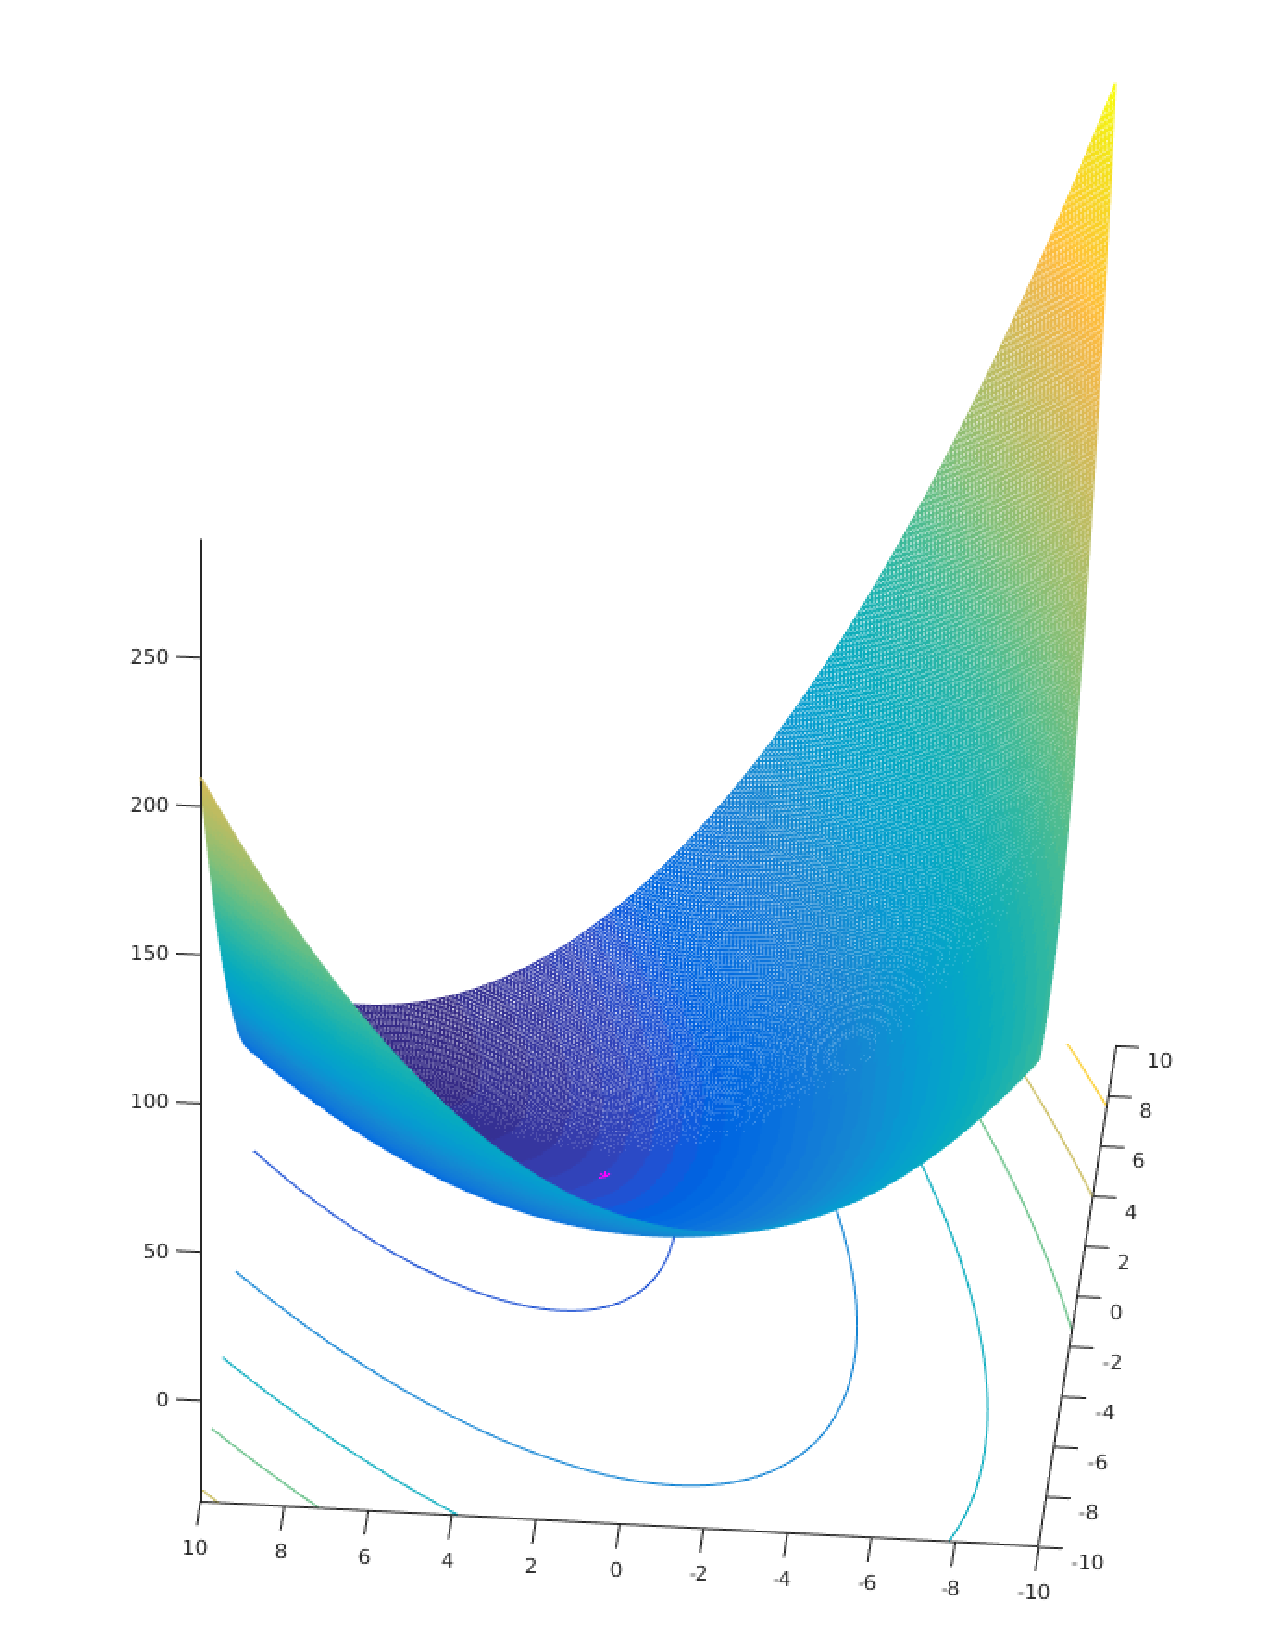
\includegraphics[width=\textwidth]{figures/qp.pdf}
        \caption{\gr{Λύση παραδείγματος του τετραγωνικού προγραμματισμού}}\label{fig:qp}
    \end{figure}
\end{otherlanguage}

\begin{otherlanguage}{english}
    \lstinputlisting[language=Matlab]{src/qp.m}
\end{otherlanguage}
